\documentclass{article}
\usepackage[T1,T2A]{fontenc}
\usepackage[utf8]{inputenc}
\usepackage[english,russian]{babel}

\usepackage[left=3cm,right=3cm,
    top=3cm,bottom=3cm,bindingoffset=0cm]{geometry}

\usepackage{graphicx}
\usepackage{color}
\usepackage{hyperref}
\usepackage{amsmath}
\usepackage{amsfonts}

\usepackage{setspace}
\usepackage{indentfirst}
\usepackage{textcomp}
\usepackage{ifthen}
\usepackage{calc}

\title{Теория Вероятностей и Математическая Статистика\\
ФИИТ, 2 курс, 4 семестр}
\author{Лекция 5}

\begin{document}
\maketitle

%\begin{center}
%    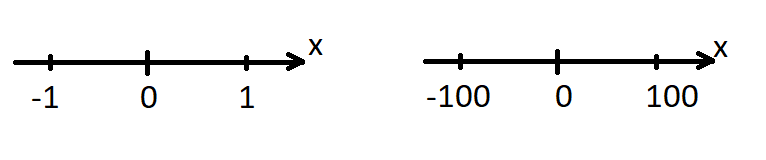
\includegraphics[scale=0.6]{9.png}
%\end{center}

\section{Характеристики распределения случайной величины}

На этой лекции мы продолжим рассмотрение характеристик распределения случайной величины.

\subsection{Квантиль распределения}

Начнем мы с непрерывной случайной величины (НСВ). Для неё квантиль определяется следующим образом:

\textbf{Определение.} Число $x_p$ -- это квантиль распределения $F(x)$ представляет собой решение уравнения:

$$F(x_p) = p,$$

и называется \textbf{квантиль уровня $p$} $(0 < p < 1)$.
\\

\textbf{Замечание 1.} В случае ДСВ квантиль определяется в зависимости от задачи.

\textbf{Замечание 2.} В электронном учебнике квантиль относится к \S5, 6, 7, там же стоит найти определения для ДСВ для каждой задачи.

\subsubsection{Квартель}

Еще одно понятие, связанное скорее с мат. статистикой. Это частный случай квантиля, рассматриваемого для величин $p = 0.25, 0.5, 0.75$.

$p = 0.25, 0.75$ -- нижний, верхний квантили.

$p = 0.5$ -- медиана распределения

\subsubsection{Пример}

В первом году средняя зарплата была меньше по сравнению с вторым годом. Инфляция при этом отсутствует. Можно ли сказать, что благосостояние/уровень жизни людей выросло?

Можно рассмотреть два случая:

\begin{enumerate}
\item У людей с низкой зарплатой зарплата стала еще ниже, а у людей с высокой зарплатой наоборот выросла. Разрыв в зарплатах стал наоборот больше.
\item У всех выросла зарплата, а значит и благосостояние.
\end{enumerate}

В общем случае, говорить об однозначном увеличении уровня жизни не приходится.

\subsubsection{Пример}

Если рассматривать пример с зарплатами в той же Москве, то мы сможем отметить, что 

\section{Дискретная случайная величина}

Напомним, что ДСВ характеризует кусочно-постоянная функция распределения, и ее можно задать рядом распределения:


\begin{quote}
$\xi \sim
\begin{pmatrix}
x_1 & x_2 & \ldots & x_n & \ldots\\
p_0 & p_1 & \ldots & p_n & \ldots
\end{pmatrix}$
\end{quote}


То есть перечислить точки разрыва функции распределения и скачки в этих точках. Условие нормировки: $\sum\limits_{i = 1}^\infty p_i = 1$.

$$M\xi = \int\limits_\mathbb{R} xdF(x) =
\sum\limits_{i = 1}^\infty x_i p_i$$

$$D\xi = \int\limits_\mathbb{R} (x - M\xi)^2 dF(x) =
\sum\limits_{i = 1}^\infty(x - M\xi)^2 p_i$$

$$M\xi^2 = \int\limits_\mathbb{R}x^2dF(x) = \sum\limits_{i = 1}^\infty x_i^2p_i$$

...

\subsection{Производящая функция неотрицательной целочисленной случайной величины}


\begin{quote}
$\xi \sim
\begin{pmatrix}
0 & 1 & 2 & \ldots & n & \ldots\\
p_0 & p_1 & p_2 & \ldots & p_n & \ldots
\end{pmatrix}$
\end{quote}


$\psi(z) = Mz^\xi \quad
\begin{cases}
z  \text{-- комплексная переменная}\\
|z| \leq 1
\end{cases}$
\\

Найдем производную по $z$:

$$\psi_z(z) = \frac{d}{dz}(Mz^\xi) = M(\frac{d}{dz}z^\xi) = M(\xi\cdot z^{\xi - 1})$$

При этом $\psi_z(1) = M\xi$
\\

Найдем так же вторую производную:

$$\psi_{zz}(z) = M(\xi(\xi - 1)z^{\xi - 2})$$

И снова посмотрим, что происходит в точке 1: $\psi_{zz}(1) = M(\xi^2 - \xi) = M\xi^2 - M\xi$

Тогда мы можем выразить $M\xi^2$:

$$M\xi^2 = \psi_{zz}(1) + \psi_z(1)$$

$$D\xi = M\xi^2 - (M\xi)^2 = \psi_{zz}(1) + \psi_z(1) - \psi_z^2(1)$$


\end{document}
